% !TEX root = ../entropy.tex

\section{Methods}%
\label{sec:methods}


\subsection{Dataset description}
\label{par:dataset_description}

We use data from Money Dashboard (MDB), a financial management app that allows
its users to link accounts from different banks to obtain an integrated view of
their
finances.\footnote{\href{https://www.moneydashboard.com}{https://www.moneydashboard.com}.}
The full dataset contains more than 500 million transactions made between 2012
and June 2020 by about 270,000 users, and provides information such as date,
amount, and description about the transaction as well as account and user-level
information.

The main advantages of the data for the study of consumer financial behaviour
are its high frequency, that it can be cheaply collected for a very large
number of users, that collection is automatic and thus less prone to errors and
unaffected by biases that bedevil survey measures, and that it offers a view of
consumers' entire financial life across all their accounts, rather than just a
view of their accounts held at a single bank, provided they added all their
accounts to MDB. The main limitation is the non-representativeness of the
sample relative to the population as a whole. Financial management apps are
known to be used disproportionally by men, younger people, and people of higher
socioeconomic status \citep{carlin2019generational}. Also, as pointed out in
\citet{gelman2014harnessing}, a willingness to share financial information with
a third party might not only select on demographic characteristics, but also
for an increased need for financial management or a higher degree of financial
sophistication. Because our analysis does not rely on representativeness, we do
not address this.\footnote{For an example of how re-weighing can be used to
mitigate the non-representative issue, see \citet{bourquin2020effects}.}
Another major limitation is imperfect transaction labelling. Money Dasbhoard
automatically classifies transaction into different categories based on
transaction descriptions and merchant information. While this classification is
quite mature and reliable for transactions with major retailers, it is
imprecise and at times incorrect for less common transactions. We discuss this
further in the next section.


\subsection{Preprocessing and sample selection}%
\label{par:preprocessing_and_sample_selection}

We use the dataset described above for a number of projects, and perform a
number of steps to create a minimally cleaned version of the dataset that is
the basis for all such projects. These steps are performed in a dedicated data
repository and not run as part of this project.\footnote{The module with all
cleaning functions is available on
\href{https://github.com/fabiangunzinger/entropy/blob/27a210e2f42dfe23a867dbc20c8ef3253d050aaa/src/data/clean.py}{Github}.}
Here, we briefly describe the main cleaning steps and their rationale. We drop
all transactions with a missing description string because these cannot be
categoriesed, and all transactions that are not automatically categoriesed by
the app. Dropping these transactions makes it likely that we will underestimate
amounts spent and saved, but minimises the risk of incorrectly classified
transactions. We also group transactions into transfer, spend, and income
subgroups, following \citet{muggleton2020evidence} to define spend subgroups
and \citet{hacioglu2021distributional} to define income subgroups.\footnote{
The precise list used to classify transactions is available on
\href{https://github.com/fabiangunzinger/entropy/blob/27a210e2f42dfe23a867dbc20c8ef3253d050aaa/src/data/txn_classifications.py}{Github}.}
Finally, we classify as duplicates and drop transactions with identical user ID,
account ID, date, amount, and transaction description. This will drop some
genuine transactions, such as when a user buys two identical cups of coffees at
the same coffee shop on the same day. However, data inspection suggests that in
most cases, we remove genuine duplicates.

To minimise the influence of outliers, we winsorise all variables at the 1
percent level or -- if we winsorise on both ends of the distribution -- at the
0.5 percent level.\footnote{The code that performs the winsorisation are
    available on
\href{https://github.com/fabiangunzinger/entropy/blob/27a210e2f42dfe23a867dbc20c8ef3253d050aaa/src/data/transformers.py}{Github}.}
We rely on winsorisation (replacing top values with percentile values) instead
of trimming (replacing top values with missing values) because data inspection
suggests that in most cases, very large (absolute) values are not the result of
data errors, which would call for trimming, but reflect genuine outcomes, which
makes winsorising appropriate because it leaves these observations in the data
while lowering their leverage to influence results.

The overall aim of sample selection is to restrict our sample to users for whom
we can observe a regular income, can be reasonably sure that they have added
all their bank account to MDB, and for whom we observe at least six months of
data. Table~\ref{tab:selection} summarises the sample selection steps we
applied, associated data losses, and the size of our final sample.

\begin{table}[ht]
\centering\footnotesize
\caption{Sample selection}\label{tab:selection}
\begin{tabular}{lrrrr}
\toprule
                                       &  Users & User-months &       Txns & Txns (m\pounds) \\
\midrule
                            Raw sample & 27,175 &     795,338 & 65,972,558 &          12,527 \\
             Drop first and last month & 26,565 &     741,170 & 64,157,932 &          12,179 \\
             At least 6 months of data & 23,238 &     732,499 & 63,592,713 &          12,074 \\
          At least one savings account & 14,315 &     473,814 & 43,983,467 &           8,898 \\
          At least one current account & 14,028 &     466,827 & 43,408,017 &           8,792 \\
At least \pounds5,000 of annual income &  5,335 &     159,663 & 16,815,335 &           3,339 \\
           At least 10 txns each month &  4,789 &     142,602 & 15,328,431 &           3,023 \\
  At least \pounds200 of monthly spend &  4,175 &     122,174 & 13,592,387 &           2,713 \\
      Complete demographic information &  3,417 &     104,660 & 11,689,245 &           2,299 \\
                       Drop test users &  3,410 &     104,307 & 11,638,106 &           2,292 \\
                           Working age &  3,345 &     102,302 & 11,465,704 &           2,241 \\
                          Final sample &  3,345 &     102,302 & 11,465,704 &           2,241 \\
\bottomrule
\end{tabular}

\tabnote{\textwidth}{Number of users, user-months, transactions, and
transaction volume in millions of British Pounds left in our sample after each
sample selection step.}
\end{table}

We start by dropping the first and last month of data for each user because we
are unlikely to observe users' complete data in these months, which might
affect selection for the criteria below. Next, we keep only users whom we
observe for at least 6 months to ensure that we have a suitable amount of data
for each user. We also require users to have at least one current and one
savings accounts to be able to oberve their spending and savings behaviour. The
next few steps are all aimed at selecting users about whom we can be reasonably
sure that they have added all their financial accounts. We thus select on
criteria we would expect to see for all such users: an annual income of at
least \pounds5,000, at least 10 monthly spending transaction, at least 4
monthly grocery transactions, and a total monthly spend of at least \pounds200.
Finally, we keep only users for whom we observe all relevant demographic
characteristics, and who are between 18 and 65 years old. The reason for the
last step is that younger users and retirees will plausibly have different
fianncial objectives than people in their working age, which is the population
we are interested about.\footnote{The code that implements the selection
criteria is available on
\href{https://github.com/fabiangunzinger/entropy/blob/c49c9c34c96d073725afd3a1494458a388d00051/src/data/selectors.py}{Github}.}


\subsection{Dependent variables}
\label{sub:dependent_variables}

Our outcome variable is biniry indicator for whether of not a user made a
payment into any of their savings account in a given month. We classify as
payments into savings accounts all savings account credits of \pounds5 or
more.\footnote{While standing order transactions are unlikely to be related to
entropy in the short-run, we do not exclude such transactions since, best we
can tell, the only account for a small fraction of total transactions.}

The reason we focus on a binary indicator is twofold: first, becaus we
hypothesis that chaotic or difficult life circumstances that are also reflected
in spending entropy might make it harder to remember to save, for which the
accurate thest is to see whether spending entropy is related to the likelihood
of making ang savings transctions. Second, research by \citet{mps2018building}
suggests that to build up sufficient emergency funds over time forming a habit
of saving regularly is more important than the specific amounts saved month to
month.

\subsection{Spending profiles}%
\label{sub:spending_profiles}

We define a user's spending profile as the distribution of the number of
spending transactionas across different spend categories. To summarise these
distributions, we calculate spending entropy, based on the formula proposed by
\citet{shannon1948mathematical}, who defines entropy as $H =
-\sum{p_i}log(p_i)$, which sums, for all possible events, the product of the
probability of an event $i$ occuring with the logarithm of that
probability.\footnote{Shannon entropy is customarily denoted as $H$ following
Shannon's own naming after Ludwig Boltzman's 1872 H-theorem in statistical
mechanics, to which it is analagous.} The base of the logarithm is often chosen
to be 2, though other choices are possible. Entropy is a cornerstone of
information theory, where it measures the amount of information contained in an
event. In the behavioural sciences, behavioural entropy has recently been shown
to predict the frequency of grocery visits and the per-capita spend per visit
\citep{guidotti2015behavioral}, the amount of calories consumed
\citep{skatova2019those}, and the propensity for financial distress
\citep{muggleton2020evidence}. In our context, we define the entropy of a
user's spending profile in a particular period as (we omit individual and time
subscripts to keep the notation simpler):

\begin{equation}
\label{equ:entropy}
H = -\sum_{c \in \setc}{p_c}log(p_c),
\end{equation}

\noindent where $\setc$ is the set of all spending categories, $p_c$ the
probability that an individual makes a purchase in spending category $c$, and
$log$ the base 2 logarithm.

Higher entropy means that transactions are more equal across different spending
categories, which makes it hard to predict the next transaction, whereas low
entropy profiles have the bulk of transactions in a few dominant categories
(such as groceries and transportation) and have relatively few transactions in
other categories.\footnote{For further discussion on how to interpret
Equation~\ref{equ:entropy}, see Appendix~\ref{sec:interpreting_entropy}.} For
simpler interpretation of our regression coefficients below, we standardise
entropy scores to have a mean of 0 and a standard deviation of 1.

One limitation introduced by the imperfect transaction labelling in the
MDB data is that entropy scores for high-entropy individuals will be biased
downwards. This happens because unlabelled transactions tend to be transactions
that are rare (i.e. not grocery or Amazon purchases), and it is high-entropy
individuals that are more likely to engage in rare transactions. Because our
analysis mainly relies on relative entropy levels, this is not of major
consequence and we do not pursue this further.

We calculate entropy based on three sets of spend categories. The first measure
is based on 9 spending categories used by \citet{muggleton2020evidence}. The
second measure is based on our own, more fine-grained, categorisation into 48
different categories.\footnote{The precise mapping from MDB transaction tags
    into 9 and 48 categories is available on Github
    \href{https://github.com/fabiangunzinger/entropy/blob/7fa9c565bf8959ea92a9d4fe2245da0864e19c27/src/data/txn_classifications.py\#L249}{here}
    and
    \href{https://github.com/fabiangunzinger/entropy/blob/7fa9c565bf8959ea92a9d4fe2245da0864e19c27/src/data/txn_classifications.py\#L503}{here},
respectively.} The third measure is based on merchant names, as labelled by
Money Dashboard.

We also calculate spending category probabilities in two different ways. To
calculate what we call ``unsmoothed'' entropy scores, we calculate the $p_c$s
in Equation~\ref{equ:entropy} as simple frequentist probabilities

\begin{equation}
    p_c = \frac{f_c}{F},
\end{equation}

\noindent where $f_c$ is the number of transactions in spend category $c$ (the
frequency with which $c$ occurs) and $F = \sum_{c \in \setc}f_c$ the total
number of spending transactions. To avoid taking the log of zero for categories
with zero transactions, the sum in Equation~\ref{equ:entropy} is taken over
categories with positive transaction counts only.\footnote{This is
    automatically handled by the entropy
    \href{https://docs.scipy.org/doc/scipy/reference/generated/scipy.stats.entropy.html}{implementation}
of Python's SciPy package, which is what we use to calculate entropy scores.}
To calculate ``smoothed'' entropy scores, we apply additive smoothing to
calculate propabilities as

\begin{equation}
    \label{equ:prob_s}
    p_c^{s} = \frac{f_c + 1}{F + |\setc|},
\end{equation}

\noindent where the size of set $\setc$, $|\setc|$, is the number of unique
spending categories. Hence, additive smoothing simply adds one to the numerator
and the number of unqiue spending categories to the denominator of the
unsmoothed probabilities. Because categories with a zero transaction count will
have a numerator of 1, the sum in Equation~\ref{equ:entropy} will be taken over
all categories.


\subsection{Summary statistics}%
\label{par:summary_statistics}

Table~\ref{tab:sumstats} provides summary statistics and
Figure~\ref{fig:sample_desc} distributions for the key variables used in our
analysis as well as for some sample demographics. Income and spending
distributions are being compared to those of the Living Cost and Food
Survey, which is the ONS's main survey on household spending. We can see that
the sample distributions broadly match the UK-wide ones but that we tend to
underestimate incomes and overestimate spend. As discussed above, our sample is
biased towards high-earning individuals, so that we would expect both income
and spend to be higher than across the whole population. The main reason this
is not the case is likely due to the imperfect identification of income
transactions in the Money Dasbhoard data.

\begin{table}[ht]
\centering\scriptsize
\caption{Summary statistics}
\label{tab:sumstats}

% Table created by stargazer v.5.2.3 by Marek Hlavac, Social Policy Institute. E-mail: marek.hlavac at gmail.com
% Date and time: Mon, Sep 26, 2022 - 09:41:15
\begin{tabular}{@{\extracolsep{5pt}}lccccccc} 
\\[-1.8ex]\hline 
\hline \\[-1.8ex] 
Statistic & \multicolumn{1}{c}{Mean} & \multicolumn{1}{c}{St. Dev.} & \multicolumn{1}{c}{Min} & \multicolumn{1}{c}{Pctl(25)} & \multicolumn{1}{c}{Median} & \multicolumn{1}{c}{Pctl(75)} & \multicolumn{1}{c}{Max} \\ 
\hline \\[-1.8ex] 
Month income & 2.77 & 2.23 & 0.00 & 1.45 & 2.18 & 3.43 & 13.69 \\ 
Has income in month & 0.98 & 0.13 & 0 & 1 & 1 & 1 & 1 \\ 
Has savings & 0.50 & 0.50 & 0 & 0 & 1 & 1 & 1 \\ 
Month spend & 2.90 & 2.50 & 0.20 & 1.37 & 2.20 & 3.49 & 16.05 \\ 
Age & 35.72 & 9.74 & 18 & 28 & 34 & 42 & 65 \\ 
Female & 0.43 & 0.49 & 0 & 0 & 0 & 1 & 1 \\ 
Urban & 0.85 & 0.36 & 0 & 1 & 1 & 1 & 1 \\ 
Unique categories (9) & 7.84 & 1.05 & 1 & 7 & 8 & 9 & 9 \\ 
Unique categories (48) & 16.54 & 4.13 & 1 & 14 & 16 & 19 & 35 \\ 
Unique categories (Merchants) & 26.78 & 9.35 & 2 & 20 & 26 & 33 & 85 \\ 
\hline \\[-1.8ex] 
\end{tabular} 

\tabnote{\textwidth}{Summary statistics for main variables used in analysis and
    user characteristics. Unique categories refer to the number of distinct
    spending categories that invididuals made purchases in within a given
    month for spending transaction categorisation based on 9 categories, 48
categories, and merchant names.}
\end{table}

\begin{figure}[ht]
    \centering
    \caption{Demographic characteristics of Money Dashboard users}
    \label{fig:sample_desc}
    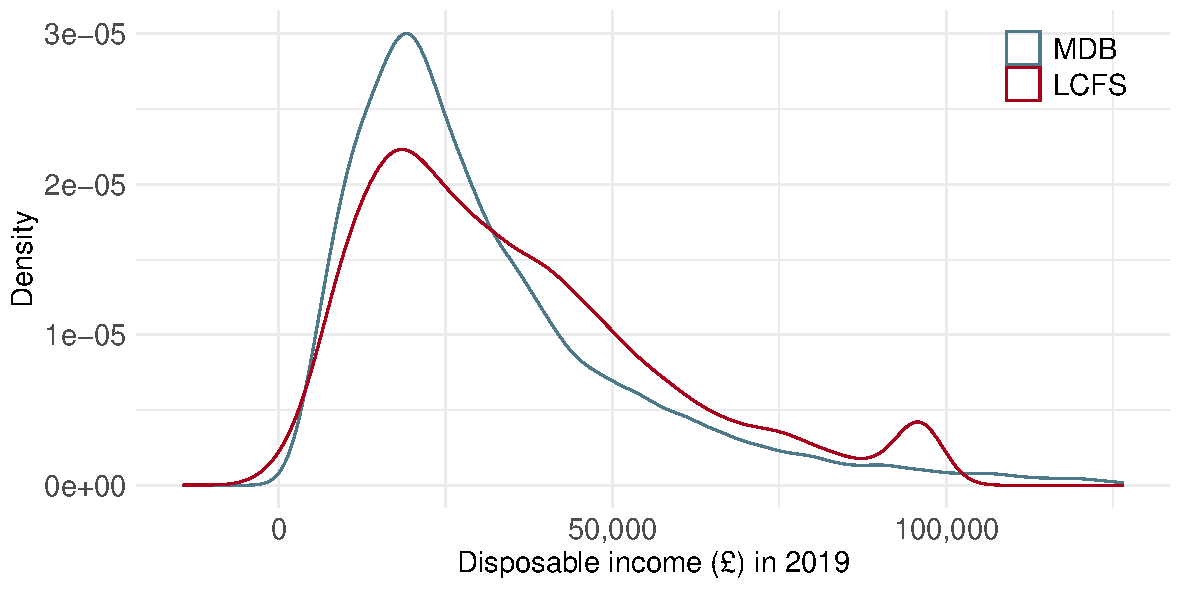
\includegraphics[width=.49\textwidth]{\figdir/year_income.pdf}
    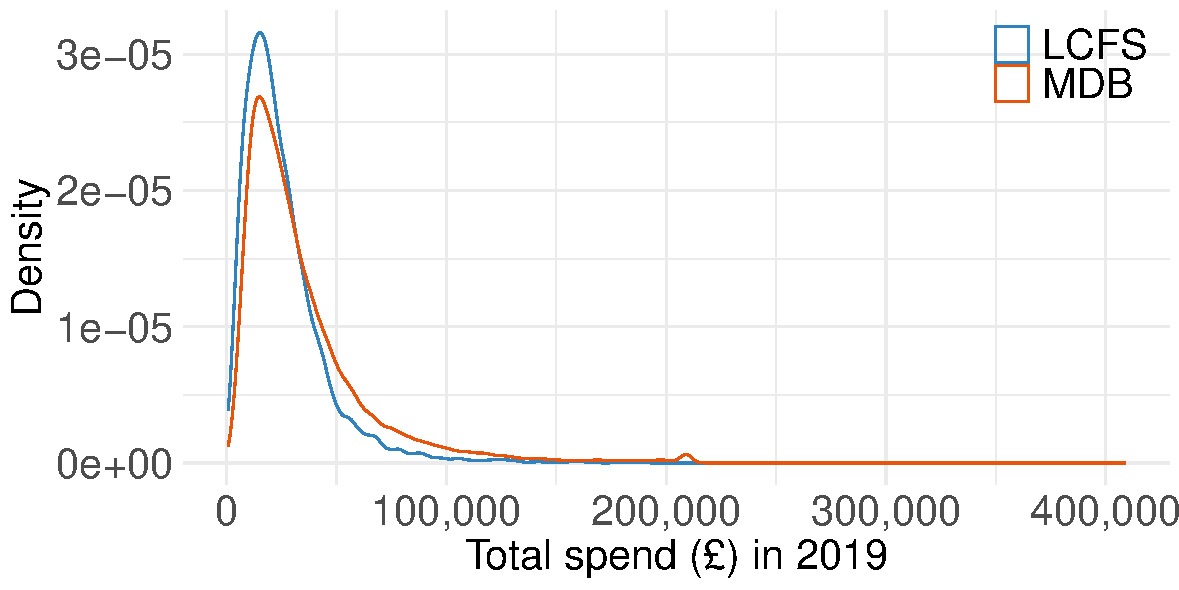
\includegraphics[width=.49\textwidth]{\figdir/year_spend.pdf}
    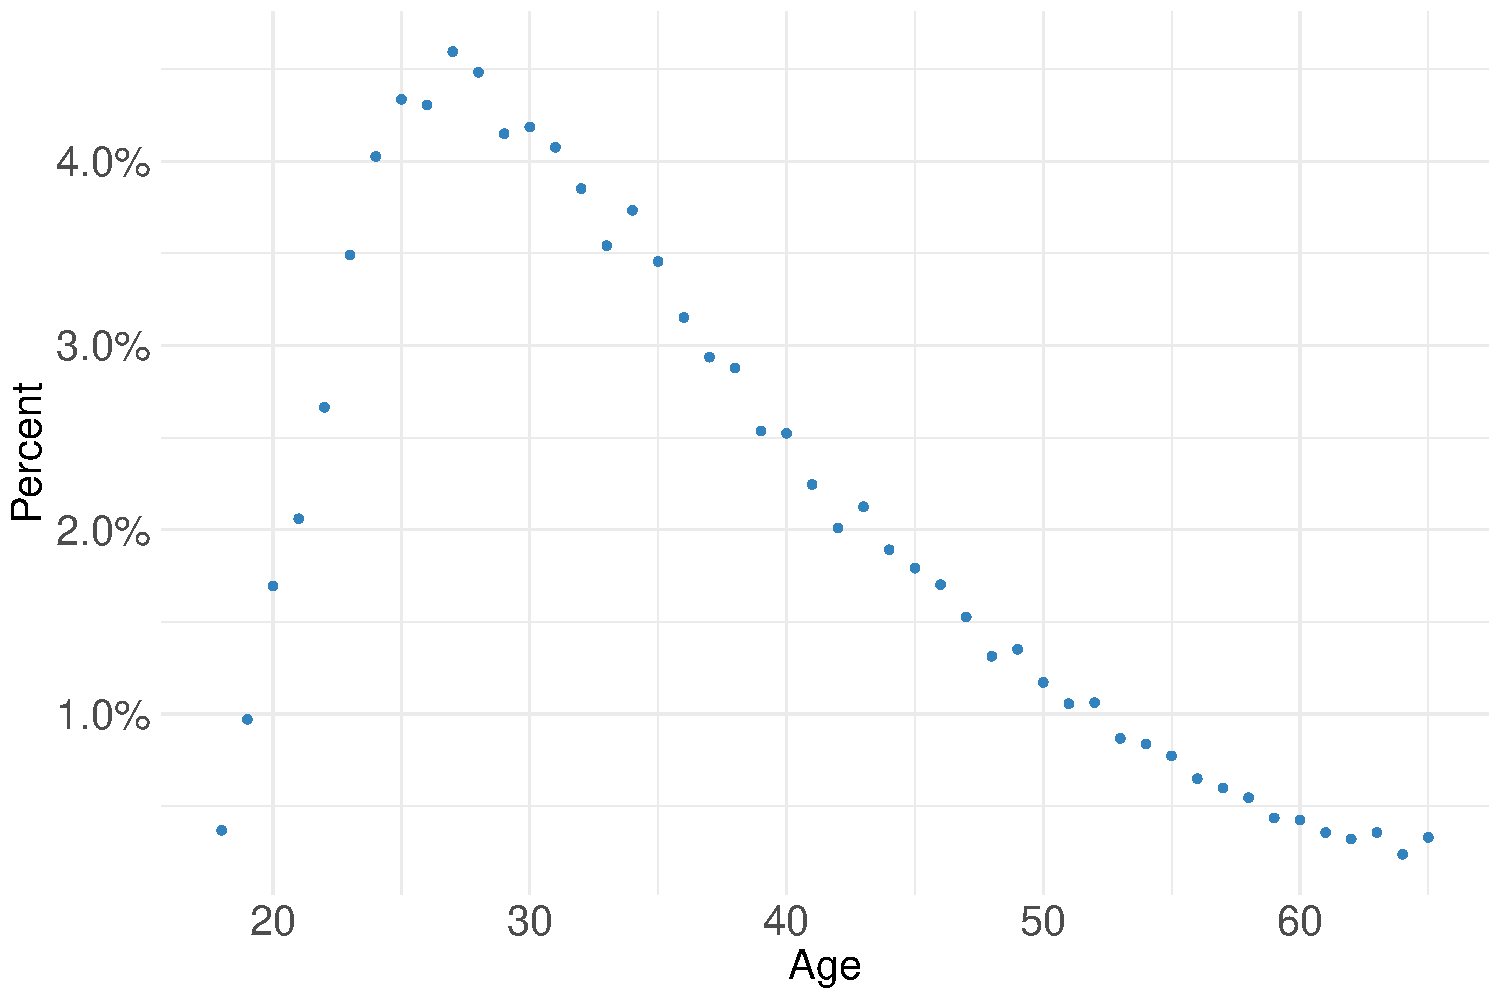
\includegraphics[width=.49\textwidth]{\figdir/age.pdf}
    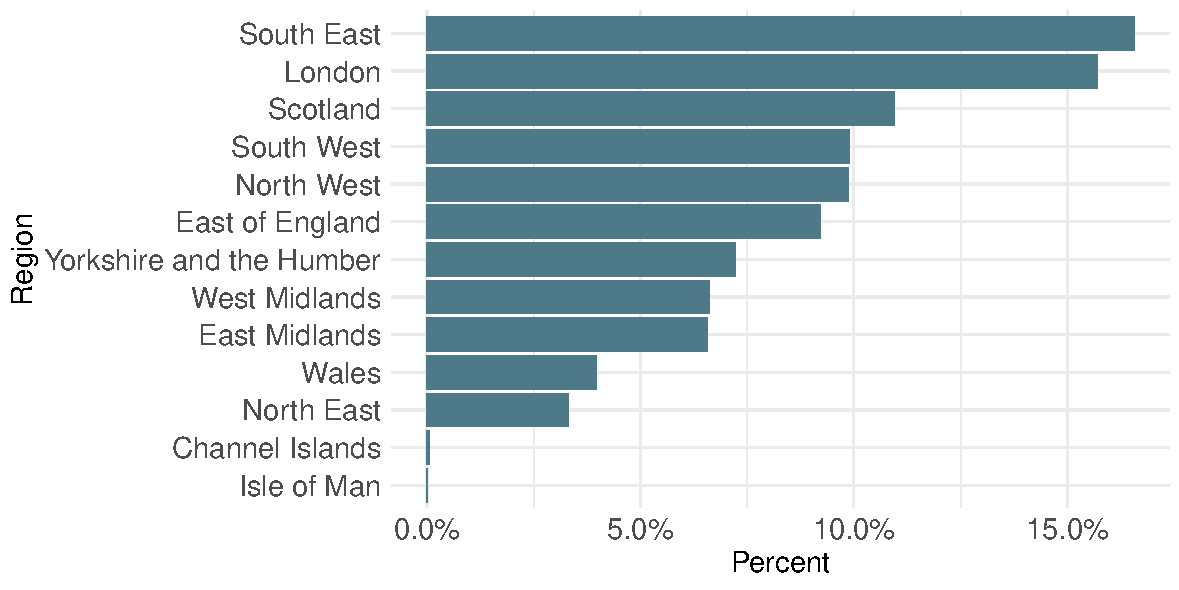
\includegraphics[width=.49\textwidth]{\figdir/region.pdf}
    \fignote{\textwidth}{The top left and top right panels show the
        distribution of disposable income and total spending in 2019,
        respectively, benchmarked against the 2018/19 wave of the ONS Living
        Cost and Food Survey (LCFS). The bottom left panel shows the
        distribution of age, the bottom right panel that of the regions.}%
\end{figure}

Individuals in our data make at least one savings transaction in half of all
observed periods, and have at least some income in 98 percent of those periods.
As discussed above, our sample is skewed towards men in their 20s, 30s, and
40s, who live in urban areas, mainly the South East of England. Mean monthly
spend is \pounds2,000 and the median is \pounds2,200, and the average
invididual spends money across 27 different merchants in 16 different
categories (of the 48 category classification).

\begin{figure}[ht] \centering \caption{Entropy distributions}
    \label{fig:entropy}
    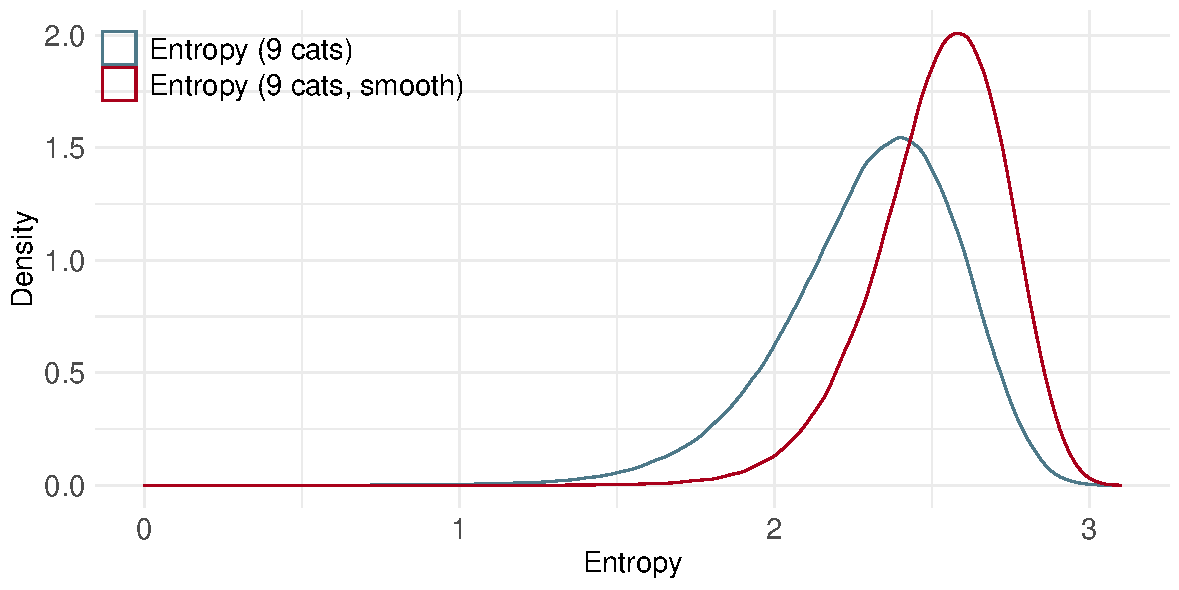
\includegraphics[width=.49\textwidth]{\figdir/entropy_tag.pdf}
    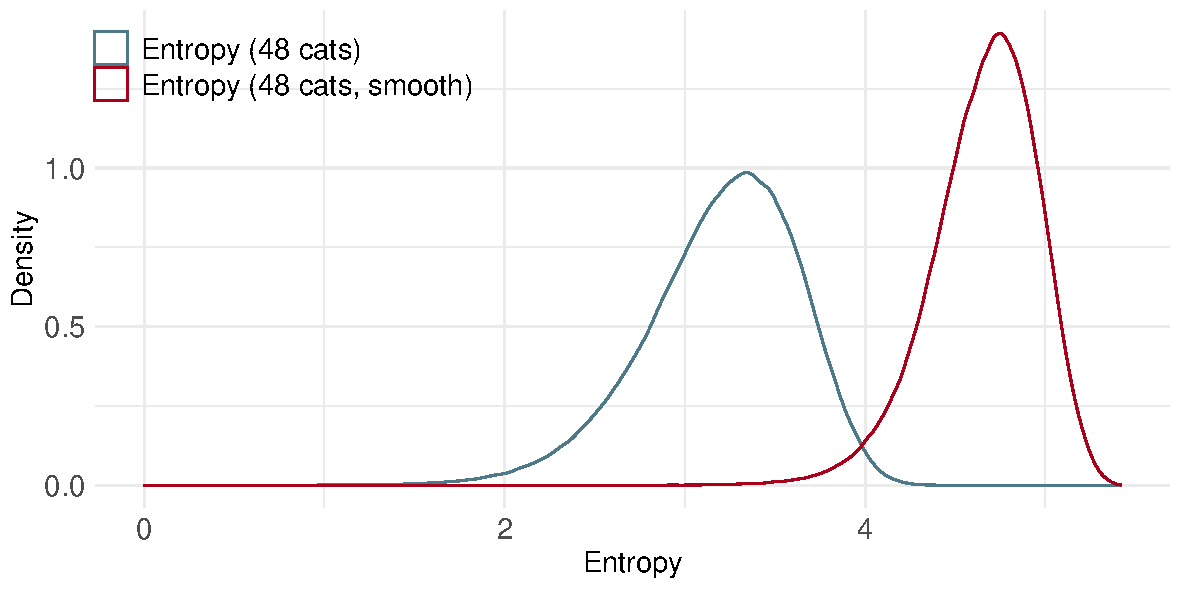
\includegraphics[width=.49\textwidth]{\figdir/entropy_tag_spend.pdf}
    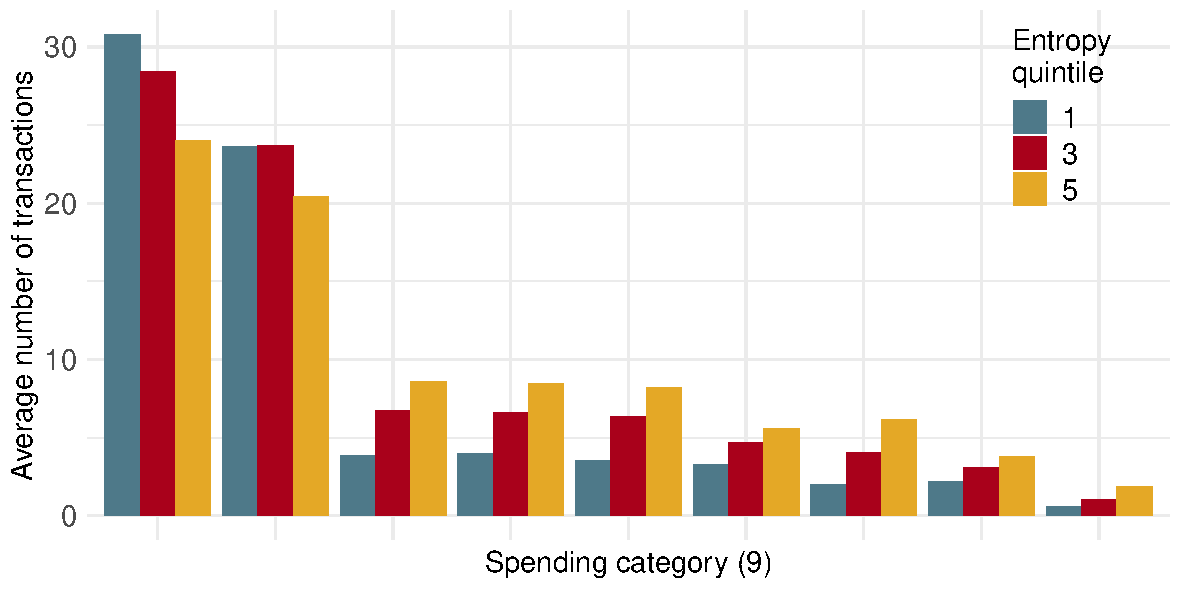
\includegraphics[width=.49\textwidth]{\figdir/spend_profile_tag.pdf}
    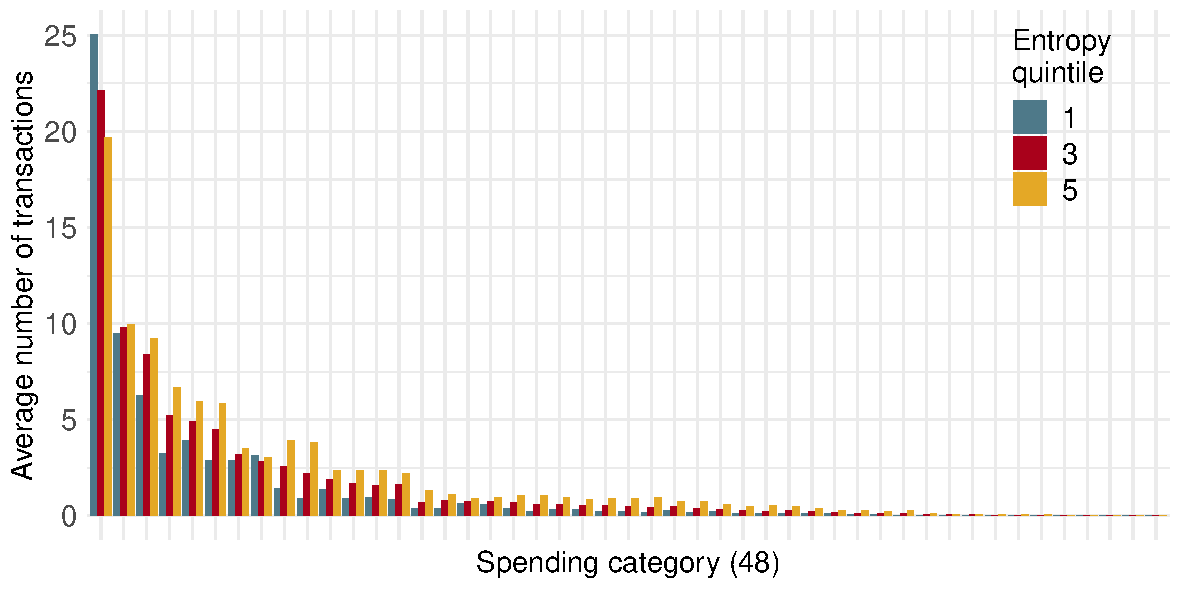
\includegraphics[width=.49\textwidth]{\figdir/spend_profile_tag_spend.pdf}
    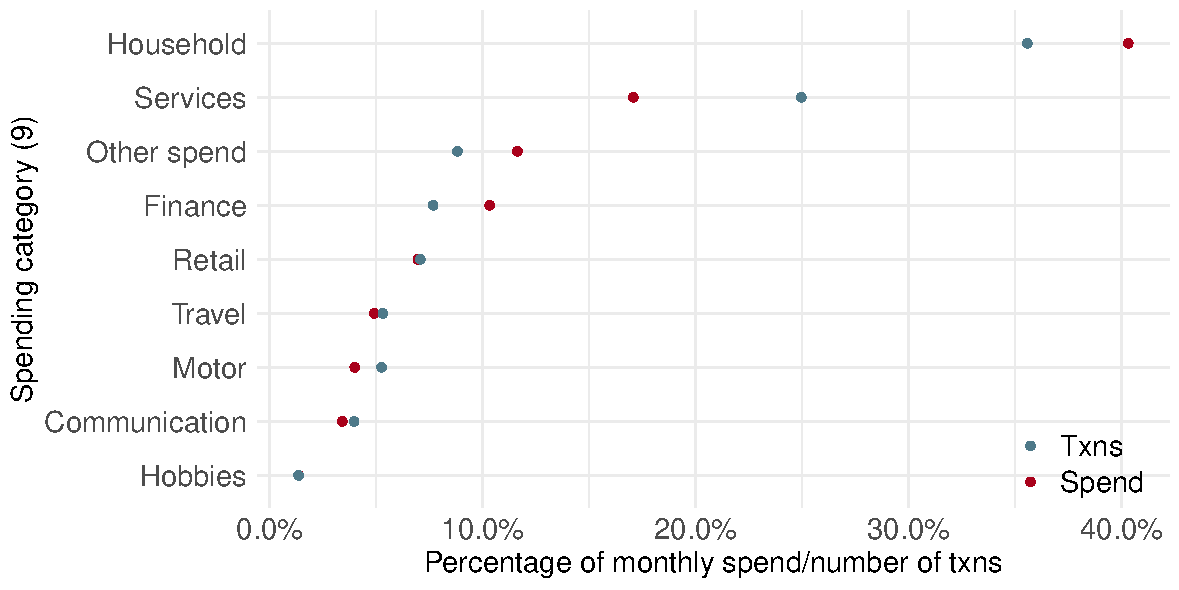
\includegraphics[width=.49\textwidth]{\figdir/breakdown_tag.pdf}
    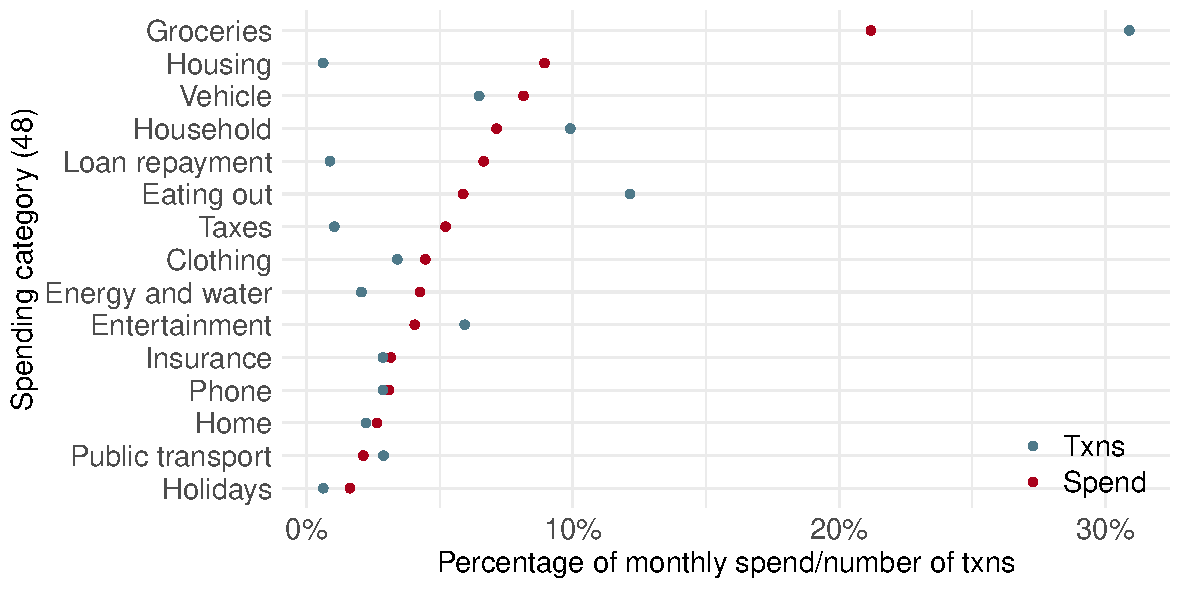
\includegraphics[width=.49\textwidth]{\figdir/breakdown_tag_spend.pdf}
    \fignote{\textwidth}{The top row shows distributions of unsmoothed and
        smoothed versions of entropy. The middle row shows associated spending
        profiles for individuals in the first, third, and fifth quintile of tne
        entropy distribution. Spending category labels are deliberately omitted
        to not overcrowd the plots and to focus on the distribution of
        transaction counts. The bottom row shows the distributions of spend and
        number of transactions that goes to the top categories. The plot on the
        left shows all 9 categories, that on the right the top 15 out of 48
        categories. The left column shows data for the 9 category
        classification, the right column data for the 48 categories
classification.}
\end{figure}

Figure~\ref{fig:entropy} shows the distributions of the unsmoothed and smoothed
version of entropy based on 9 and 48 spending categories, in the top row, the
associated average spending profiles for individuals in the first, third and
fifth quintiles in the middle row, and an overview of the main categories
individuals spend on in the bottom row. The entropy distributions are bounded
on the right by the maximum entropy value, given by the value for a discrete
uniform distribution with 9 or 48 distinct values,\footnote{For instance, the
upper bound for the 9 category variable is $9 \times
\left(\frac{1}{9}\right)log_2\left(\frac{1}{9}\right) \approx 3.17$.} and on
the left by zero, the value for cases where an individual makes all spending
transactions in a single category. The different effect of smoothing on the two
variables is a result of the different number of categories with counts of
zero.

The spending profiles in the middle row show that higher entropy individuals
make both fewer transactions in high-count categories and more transactions in
low-count categories. The spend profile based on the 48 category classification
also shows that spend counts follow approximately a power law distributions,
with very few of the 48 categories accounting for the large majority of
transactions.

The relative ordering of the top spending categories based on the 48 category
classification is about as expected, as are the relationship between the number
of transactions and spend: there are, for instance, a large number of
relatively low value transactions and meals eaten out (which includes snacks
and coffee) and a very small number of high value transactions for housing. The
proportion of spend that goes towards housing, less than 10\%, is clearly an
underestimate, however, and reflects the challenge and imperfect nature of
automatic transaction labelling in our data that we discussed above.

\subsection{Estimation}%
\label{sub:estimation}

To estimate the relationship between spending entropy and savings behaviour we
estimate fixed-effect models of the form: 

\begin{equation}
    \label{equ:model}
    y_{i,t} = \alpha_i + \lambda_t + \beta H_{i,t} + x^\prime_{i,t} \delta +
    \epsilon_{i,t},
\end{equation}

\noindent where $y_{i,t}$ is an indicator variable equal to one if individual
$i$ made at least one transfers to any of their savings account in year-month
period $t$ and zero otherwise, $H_{it}$ is $i$'s spending entropy in year-month
period $t$, $x_{i,t}$ a vector of control variables, $\alpha_i$ an individual
fixed effect, $\lambda_t$ a year-month fixed effect, and $\epsilon_{i, t}$ the
error term.

The vector of controls includes month spend, month income, an indicator for
whether a user had positive income in a given month, and income
variability, calculated as the standard deviation of month income over the
previous 12 months.

Note that while we might in principle be worried about reverse causality, since
making payments into savings accounts might lead to a non-zero count in an
additional spend category and thus change entropy, this is not a concern here.
As discussed in Section~\ref{sub:dependent_variables} and
Section~\ref{sub:spending_profiles}, we define savings as inflows into savings
accounts and define entropy based on the classification of spend transactions
on current accounts. If a user pays money from their current into one of their
savings account, such a transaction will usually be labelled in their current
account as a transfer rather than a spending transaction, and thus not enter
the calculation of their entropy score. In Appendix~\ref{sub:endogeneity}, we
provide robustness checks using lagged entropy scores, which produces very
similar results.

